\documentclass[border=8pt]{standalone}
\usepackage{mathpazo}
\usepackage{tikz}
\usetikzlibrary{arrows.meta}

\definecolor{stblue}{HTML}{7B97AD}
\definecolor{rwgold}{HTML}{B8995E}
\definecolor{sage}{HTML}{7A9A7E}
\definecolor{terracotta}{HTML}{C47A6A}
\definecolor{dkbrown}{HTML}{3D3530}
\definecolor{wmgray}{HTML}{7B7067}
\definecolor{lavender}{HTML}{907EA0}
\definecolor{sagefill}{HTML}{E8F0E9}
\definecolor{bluefill}{HTML}{E8EDF2}
\definecolor{lavfill}{HTML}{EDE8F0}

\begin{document}
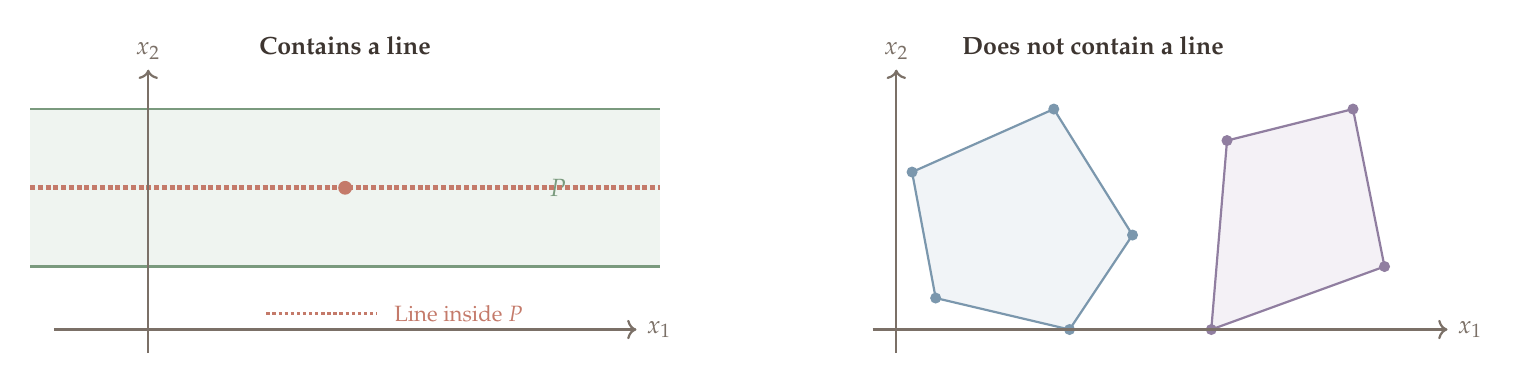
\begin{tikzpicture}

% ===== Left panel: Contains a line =====
\begin{scope}[shift={(0,0)}]
  % Title
  \node[font=\bfseries\small,dkbrown] at (2.5,3.6) {Contains a line};

  % Infinite strip: 1 <= x2 <= 3
  \fill[sagefill,opacity=0.7] (-1.5,0.8) rectangle (6.5,2.8);
  \draw[sage,thick] (-1.5,0.8) -- (6.5,0.8);
  \draw[sage,thick] (-1.5,2.8) -- (6.5,2.8);

  % Label
  \node[sage,font=\small] at (5.2,1.8) {$P$};

  % Dashed line through the strip
  \draw[terracotta,densely dotted,line width=1.8pt] (-1.5,1.8) -- (6.5,1.8);
  \fill[terracotta] (2.5,1.8) circle (2.5pt);

  % Legend
  \node[terracotta,font=\footnotesize,anchor=west] at (3.0,0.2) {Line inside $P$};
  \draw[terracotta,densely dotted,line width=1.2pt] (1.5,0.2) -- (2.9,0.2);

  % Axes
  \draw[->,wmgray,thick] (-1.2,0) -- (6.2,0) node[right,font=\small] {$x_1$};
  \draw[->,wmgray,thick] (0,-0.3) -- (0,3.3) node[above,font=\small] {$x_2$};
\end{scope}

% ===== Right panel: Does not contain a line =====
\begin{scope}[shift={(9.5,0)}]
  % Title
  \node[font=\bfseries\small,dkbrown] at (2.5,3.6) {Does not contain a line};

  % Bounded polytope 1 (blue)
  \fill[bluefill,opacity=0.6] (0.5,0.4) -- (2.2,0) -- (3.0,1.2) -- (2.0,2.8) -- (0.2,2.0) -- cycle;
  \draw[stblue,thick] (0.5,0.4) -- (2.2,0) -- (3.0,1.2) -- (2.0,2.8) -- (0.2,2.0) -- cycle;
  \fill[stblue] (0.5,0.4) circle (2pt);
  \fill[stblue] (2.2,0) circle (2pt);
  \fill[stblue] (3.0,1.2) circle (2pt);
  \fill[stblue] (2.0,2.8) circle (2pt);
  \fill[stblue] (0.2,2.0) circle (2pt);

  % Bounded polytope 2 (lavender)
  \fill[lavfill,opacity=0.6] (4.0,0) -- (6.2,0.8) -- (5.8,2.8) -- (4.2,2.4) -- cycle;
  \draw[lavender,thick] (4.0,0) -- (6.2,0.8) -- (5.8,2.8) -- (4.2,2.4) -- cycle;
  \fill[lavender] (4.0,0) circle (2pt);
  \fill[lavender] (6.2,0.8) circle (2pt);
  \fill[lavender] (5.8,2.8) circle (2pt);
  \fill[lavender] (4.2,2.4) circle (2pt);

  % Axes
  \draw[->,wmgray,thick] (-0.3,0) -- (7.0,0) node[right,font=\small] {$x_1$};
  \draw[->,wmgray,thick] (0,-0.3) -- (0,3.3) node[above,font=\small] {$x_2$};
\end{scope}

\end{tikzpicture}
\end{document}
